\chapter[piet-editorを作ったので宣伝]{piet-editorを作ったので宣伝}

周りの人がよくPietのエディタを作っているので
\footnote{Pietのエディタを作った話(\url{http://www.slideshare.net/KMC_JP/piet-46068527}) Pidet \url{https://github.com/dnek/Pidet}}
\footnote{Muratam/UltraPiet \url{https://github.com/Muratam/UltraPiet}}、
一度ぐらい作っておかないといけないかな と思って作りました。

\url{https://piet-editor.github.io/}です。
スマートフォンでもPietの実行ぐらいはできそうな感じですが、全ての機能を利用するにはPCから実行してください。

ブラウザで描いたり実行したり共有したりできるようにと作りました。
描く、実行、ステップ実行、import、exportと一応一通りできます\footnote{undoがまだできないので実装しないと……。}。
下に画面のスクリーンショットが出ていますが、Shareという所からURIを作ることによって、
ブラウザで描いたPietをURIにして共有することもできます。
例えば、\href{https://piet-editor.github.io/#code=H4sIAMg7XVgCA0tMTM9OS6nx9g4PD0-q8U4MT87Kr0lMTPT29gYAp0dBWRsAAAA@&width=6&height=4}{https://piet-editor.github.io/\#code=H4sIAMg7XVgCA0tMTM9OS6nx9g4PD0-q8U4MT87Kr0lMTPT29gYAp0dBWRsAAAA@\&width=6\&height=4}というURI……は長いので、
短縮したもの\url{http://bit.ly/2inLPSZ}を辿ると、
適当に描いた`@'を出力するPietが表示されると思います。

こんな感じの画面が出たりするはずです\footnote{画面は開発中のものです。大きな変更が入る可能性がありますが、何も出ないとか明らかなバグみつけたら教えてください……。
\url{https://github.com/piet-editor/piet-editor/issues/new} or なんかリプライででも}。
CSSをまだ全く書いていないので(あとデバッグ用の出力が下のほうに出ていますし)、まだUIがわかりづらいかもしれません。
\begin{center}
  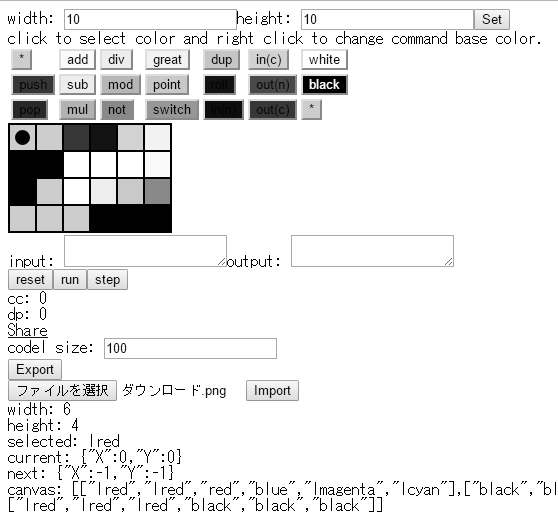
\includegraphics{images/editor_g.png}
\end{center}
Pidet\footnote{\url{https://github.com/dnek/Pidet}}
を触っていたらなんとなくわかるような雰囲気にしたつもりですが\footnote{Pidet触ったことが無くてもぜんぜん良いんですが、PietそのものについてはPietのエディタを作った話(\url{http://www.slideshare.net/KMC_JP/piet-46068527})の46ページぐらいまでの内容(Pietの言語仕様についての説明です)は前提にさせてもらいたいです……。
そもそもPietの仕様が前提に無い人がこの本読んで嬉しいんだろうか……とか考え出すと、そもそも誰がこれを読む????? みたいなきもちになってくるのでよくないですね。}、
ブラウザだけでPietに入門できてうれしい みたいな気持ちの人が表われるようにと作った点もあるのでよくないですね。
もうちょっとUIに説明入れないと……。

実装については一応Pietの本を名乗っているので詳しくは省きますが、React+es6で、piet-testutils\footnote{\url{https://github.com/nna774/piet-testutils}}からインタプリタ部分を切り出して、piet-interpreter\footnote{\url{https://github.com/nna774/piet-interpreter}}というnpm moduleにしたりして使い回したりしたので、意外とすぐにできたという感じです。

一応既にPietDev\footnote{\url{http://www.rapapaing.com/blog/?page_id=6}}のような物が既に存在していたりするのですが、
『Pietのエディタを作った話』でも上げられていたような不満点があり、また、上記のように既存のコードを使い回せる部分が多いと思ったので作りました
\footnote{既存のコードに微妙なコーナーケースでのバグがあったりしてハマったりもしたのですが……}。

アイコンである\url{http://bit.ly/2io3oCr}や、さっきの\url{http://bit.ly/2inLPSZ}を開いてポチポチしたりするなどして是非一度遊んでみてください
(そして是非改善点やバグなどを見付けたら教えてください)。
